\section{Systems}
\subsection{Design and architecture} \label{Design of the CSharp-MiniTwit application}
% We have decided to convert the given source code into an application called 'Csharp-Minitwit' written in C\#. We have chosen C\# for its well documented ecosystem and robustness, due to it being statically and strongly typed, and we have chosen to build our app using the NET 8.0 runtime, as it is the latest long-term supported release (end of support Nov. 2026)\cite{netcoresupport}.

% The application itself requires a database for storing users, messages, followers and metadata. For this we have chosen to connect to a PostgreSQL using Entity Framework Core (an ORM), making subsequent database alterations and migrations easy. In Figure \ref{fig:architecture} we have shown the architecture of the system. 

We have developed 'Csharp-Minitwit' using C\# and the .NET 8.0 runtime, chosen for its strong, statically typed ecosystem and long-term support.\cite{netcoresupport} The application uses the ASP.NET Core framework\cite{aspnetcoreintro2023}, with razor pages for rendering HTML pages, and we are following a Model-View-Controller (MVC) pattern and dependency injection, for easier maintainability and testability. We use PostgreSQL with Entity Framework Core for database management (an ORM), making subsequent database alterations and migrations easy. Below we will show the design and architecture of our system through the module viewpoints presented by Christensen et al.\cite{viewpoint} 

\subsubsection{Module Viewpoint}
In 'Csharp-Minitwit', the main modules include controllers, Models, Views, Services and Repositories. In Figure X, the dependencies between the modules can be seen. If we look into xxxx, it is apparent that the controller is heavily dependent on other modules, as illustrated in figure xx. 

\todo{Package diagram}

\subsubsection{Component \& Connector Viewpoint }
We will cover the Component \& Connector viewpoint under point 1.3. Elaborating on the interaction of subsystems.  

\subsubsection{Allocation Viewpoint}
% The purpose of the allocation viewpoint is to show how software elements are mapped to platform elements. 
%Figure \ref{fig:architecture} shows a full view of our deployment.
Figure \ref{fig:architecture} shows the infrastructure in our system.
It can be seen, how he application is hosted on DigitalOcean. We have a Docker Swarm Cluster to orchestrate containers and use Terraform for automating provisioning and configuration of the infrastructure.

\todo{elaborate on the elements. Refer directly to the figure}

\begin{figure}[H]
    \centering
    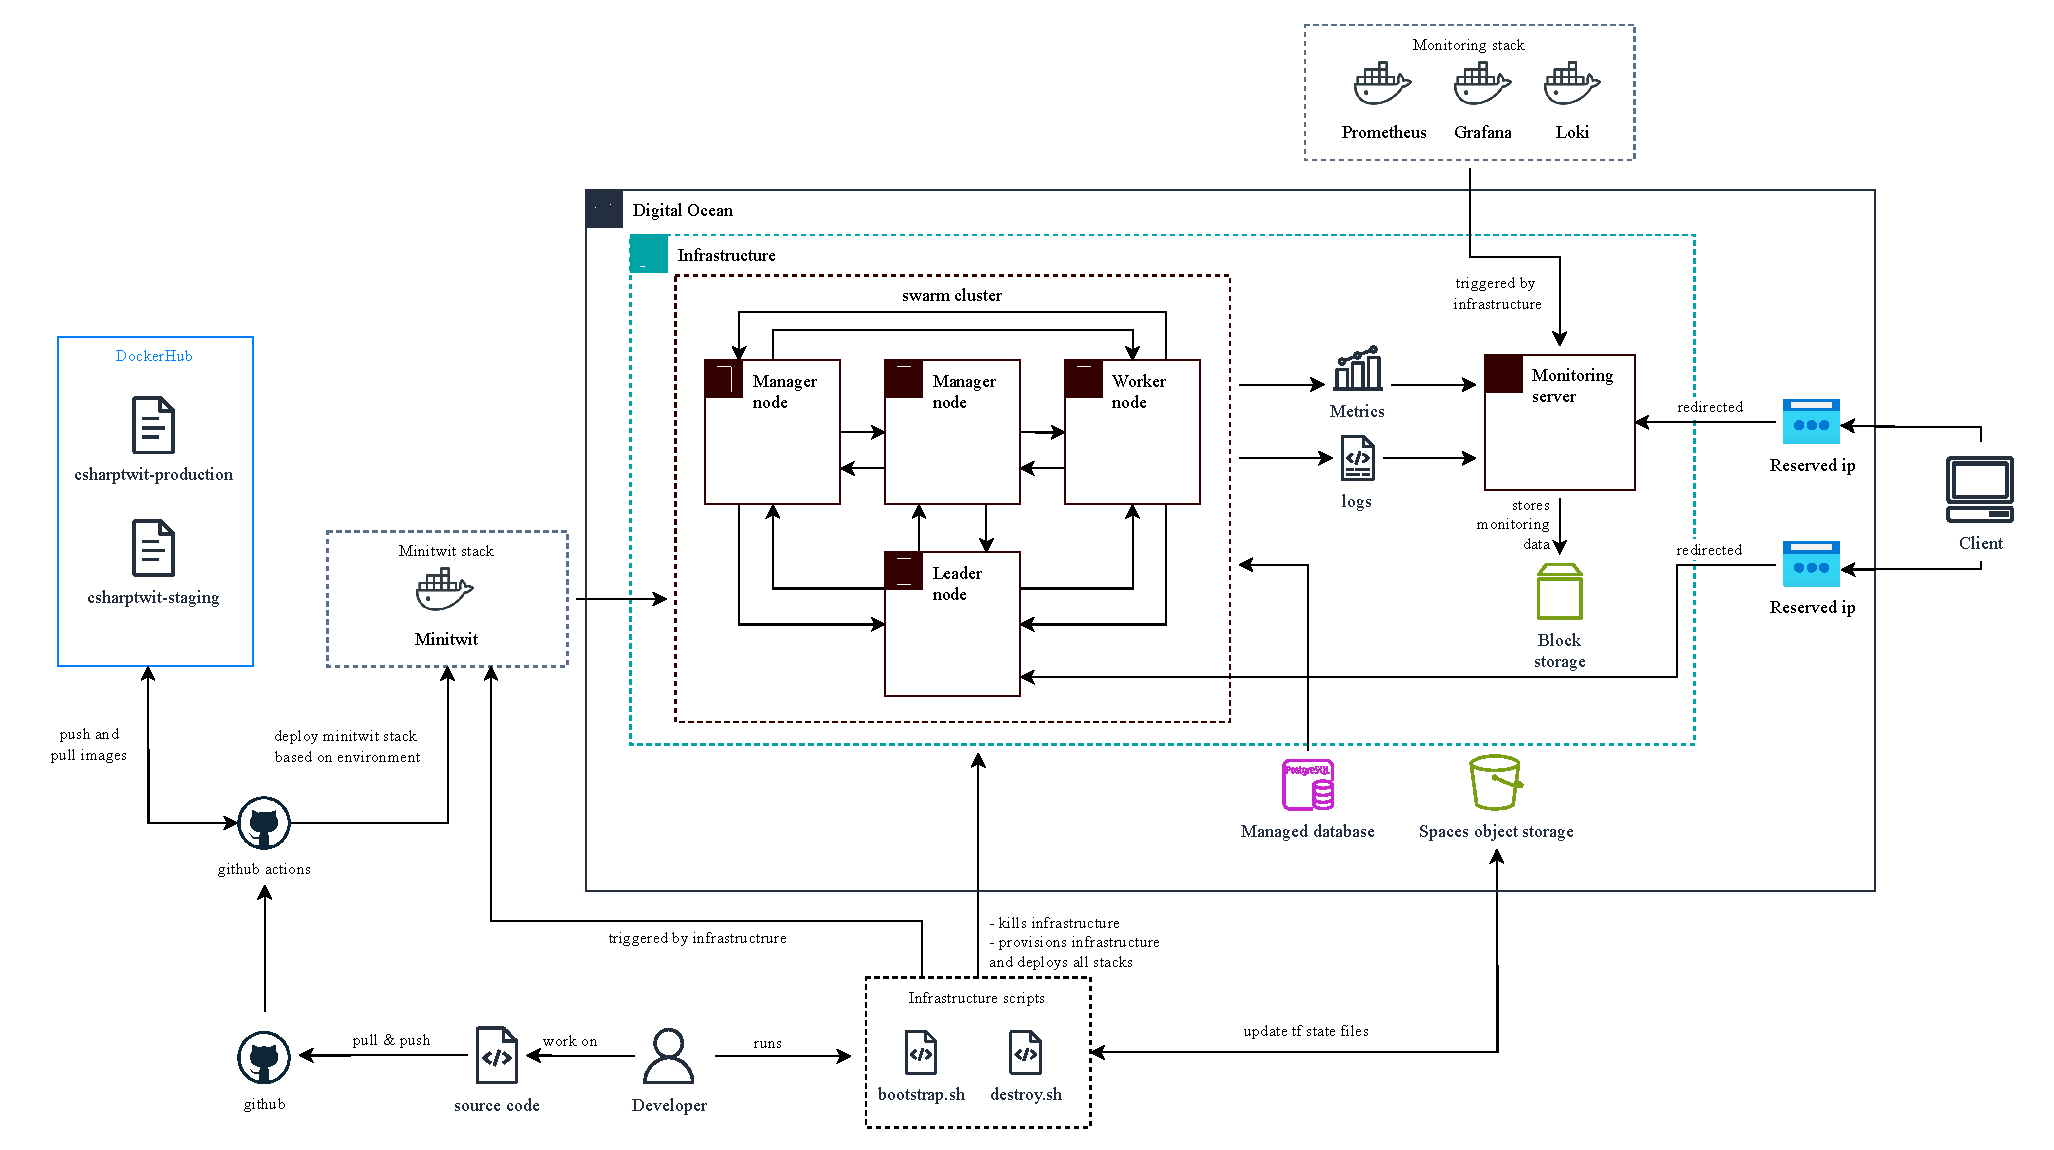
\includegraphics[width=1.0\textwidth]{figures/devops-architecture-architecture_v2.pdf}
    \caption{System Architecture Diagram, see large scale in Appendix \ref{apendix:systems-architecture}}
    \label{fig:architecture}
\end{figure}

\subsection{Dependencies and technologies}
\subsubsection{Application Dependencies}
% probably this info can be presented in tables with three columns (dev, staging, prod) and "X" pointing to the environment in which each is used.
Dependencies are handled using dotnet's package manager, NuGet:
\begin{itemize}
    \item Npgsql.EntityFrameworkCore.PostgreSQL 
    \item OpenTelemetry.Exporter.Prometheus.AspNetCore (exports telemetry data to Prometheus)
    \item OpenTelemetry.Extensions.Hosting
    \item Microsoft.EntityFrameworkCore (ORM)
    \item Serilog (structured logging library)
    \item Swashbuckle.AspNetCore (auto-generated Swagger documentation)
\end{itemize}

\subsubsection{Technologies used}
A quick overview of the technologies used:
\begin{itemize}
    \item \textbf{GitHub}: Code repository, versioning and project management.
    \item \textbf{SonarCloud}: ensuring quality in the code.
    \item \textbf{CodeClimate}: Quality analysis.
    \item \textbf{dotnet format}: Automatic formatting.
    \item \textbf{HadoLint}: Linting Docker file.
    \item \textbf{Digital Ocean}: hosting of virtual servers, databases and volumes.
    \item \textbf{Terraform}: provisioning and management of infrastructure on Digital Ocean.
    \item \textbf{Docker}: containerization of the application for deployment.
    \item \textbf{Prometheus}: monitoring system and time series database that collects metrics.
    \item \textbf{Loki}: log aggregation system integrated with Grafana for viewing logs.
    \item \textbf{Grafana}: visualization of metrics and logs.
\end{itemize} 
\subsubsection{Versioning and CI/CD}
% The application is versioned, tested, quality assured and deployed using
% GitHub. Our group has been following the Gitflow workflow to avoid merge conflicts, and ensure tractability. Gitflow also allows us to have a 'develop' and a 'main' branch, enabling us to easily set up a staging server, for integration testing.

% Our GitHub repository is also used for project management, creating issues and documentation. Deploying our application to our servers is done using GitHub actions, creating Docker images and pushing them to the relevant environment. GitHub actions also runs unit tests, formats our source code using 'dotnet format' and analyzes it using SonarCloud and CodeClimate.\\\\
% GitLab would have been a good alternative, however the whole group already have GitHub accounts and use it for personal projects — GitLab supports all the same features but is known for having a stronger focus on DevOps and CI/CD\cite{gitlabvsgithub}. GitLab allows for free self-hosting. 

Our CI/CD pipeline uses GitHub for versioning, issue tracking, and project management. GitHub Actions automate deployments, run unit tests, format code with 'dotnet format', and analyze it with SonarCloud and CodeClimate. We use Gitflow workflow for branch management, supporting staging and production environments.

\subsubsection{Cloud provider}
% We have chosen DigitalOcean as our cloud provider, running our application on provisioned virtual machines that we manage our selves. DigitalOcean has been chosen for the sole reason that they offered \$200 in credits for students — enough for the entire project.\newline 
% Since we are not using managed application services, pretty much any cloud provider would suit our needs. Had we gone with managed services, Azure would have been a good alternative due to its integrations for ASP.Net.

DigitalOcean hosts our virtual machines, chosen for its \$200 credits for students. Any cloud provider could suffice as we manage our VMs independently.

\subsubsection{Provisioning}
% For provisioning we use Terraform, which has been chosen specifically for it being declarative. The Terraform scripts are run using the 'bootstrap.sh' script, which takes a single parameter; 'production' or 'staging'. This in turn provisions our entire system (except the database) and pushes the corresponding docker image to the Docker Swarm.

Terraform, chosen for its declarative nature, provisions our infrastructure. The 'bootstrap.sh' script, which takes a single parameter; 'production' or 'staging'. This in turn provisions our entire system (except the database) and pushes the corresponding docker image to the Docker Swarm.

\subsubsection{Database}
As mentioned, the application uses a PostgreSQL database. We have opted to go with a managed database, for simplicity and to delegate reliability issues to DigitalOcean. A single vertically scaled database will be able to handle many concurrent users. If we needed to scale up substantiably, we would likely have to switch to a specialized distributed database system like Kafka, which the real X uses\cite{kafka}.

% We use a managed PostgreSQL database for simplicity and reliability. For scaling, we would consider a distributed database system like Kafka.

% \subsubsection{Monitoring and logging}
% We use Prometheus in a pull-based configuration for business monitoring. This was implemented as part of the exercises and has been kept for that reason. We also use DigitalOcean's website for infrastructure monitoring, displaying CPU, memory and disk usage. We have no alarms / emails set up.\\\\
% For logging we use Loki, which is inspired by Prometheus and chosen for that same reason\cite{Loki}.\\\\
% Grafana is used to display Prometheus data as a dashboard, and to query the logs from Loki.

% We use Prometheus for monitoring, DigitalOcean for infrastructure monitoring, it was introduced in exercises, and has been kept since. We have Loki for log aggregation, and Grafana for data visualization. Loki is inspired by Prometheus and chosen for that same reason\cite{Loki}.

\subsubsection{Containerization and container orchestration}
% The application is built as a Docker image through the CI/CD chain. From there it is deployed to an instance of Docker Swarm, using a compose file that connects our application with a Prometheus container. This setup has 2 replicas running on the swarm, more could be appliued, to scale the application if there is an increase in requests.\\
% The Grafana server is setup using standard Grafana, Prometheus and Loki images, composed together in a \texttt{docker-compose.yml}.\\\\
% The Docker Swarm is setup with 1 leader node, 2 manager nodes and 1 worker node. We only have a single worker node, as we have hit a max number of VMs, and we want to have both a staging and a production environment. To enable the leader node to crash and its role be taken by another node, it is required to have 2 manager nodes.\\\\

The application is containerized with Docker and deployed using Docker Swarm, set up with 1 leader node, 2 manager nodes, and 1 worker node. Grafana, Prometheus, and Loki are managed with a \texttt{docker-compose.yml} file.


\subsection{Interactions of subsystems}
Incoming requests to the application are handled by either the \texttt{APIController} or the \texttt{HomeController}. Both provide similar endpoint logic but are meant to be used by the simulator and regular users respectively. A request's path will match a specific endpoint, prompting the application to perform a corresponding database operation. For instance a POST request to \textit{/login} will invoke the \texttt{GetByUsername} method from the \texttt{userRepository} and request the user information through an SQL SELECT query. The ORM will map the results back to C\# objects, which the controller returns in the HTTP response to the user. 
Alng with this Prometheus and Grafana collect metrics to visualize. Data from logging is aggregated through Loki and Serilog. Below are two sequence diagrams showing how a user and the simulator interacts with our subsystems.\newline

In Figure \ref{fig:homecontroller} is a sequence diagram showing how a user successfully follow another user and gets a response from the system.\newline

\begin{figure}[H]
  \begin{center}
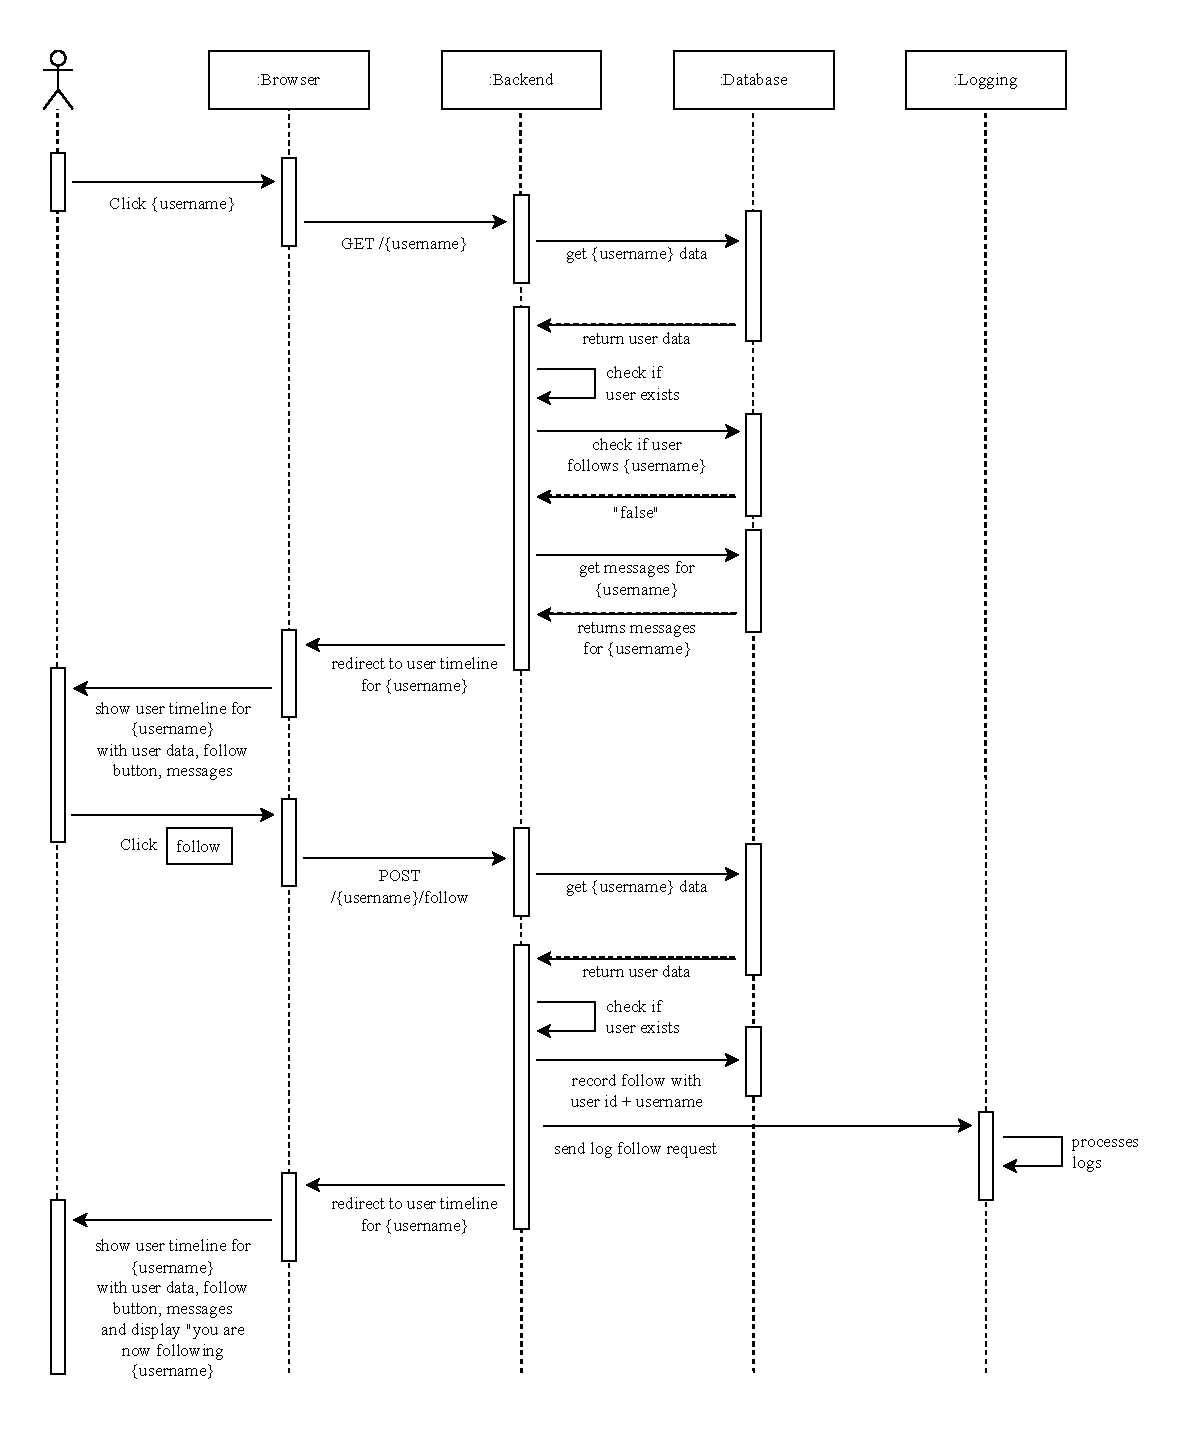
\includegraphics[width=\textwidth]{images/figures/Sequence-client.pdf}
    \caption{Sequence diagram of a successful follow scenario from user perspective.}
    \label{fig:homecontroller}
  \end{center}
\end{figure}

In Figure \ref{fig:apicontroller} is a sequence diagram illustrating how a request from the simulator is handled in the system.\newline

\begin{figure}[H]
  \begin{center}
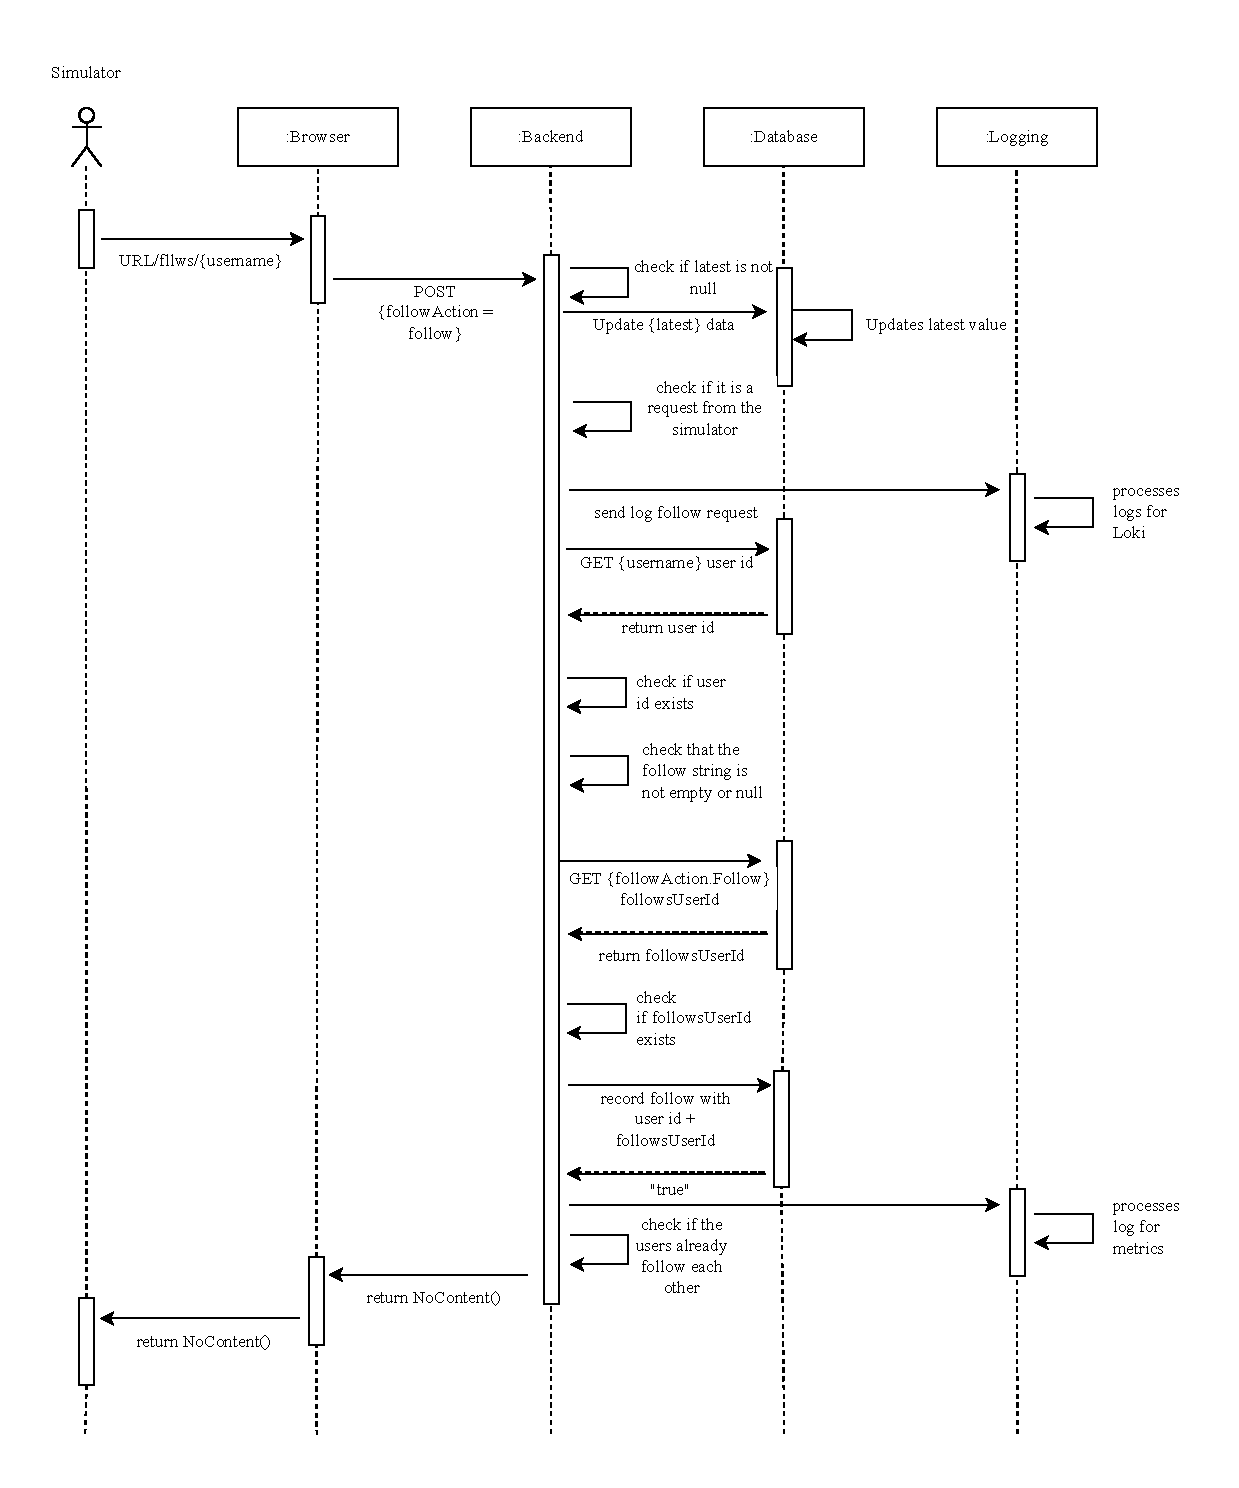
\includegraphics[width=\textwidth]{images/figures/Sequence-api.pdf}
    \caption{Sequence diagram of a successful follow scenario from the simulator over the API.}
    \label{fig:apicontroller}
  \end{center}
\end{figure}


\subsection{Current state of the systems}
The application is currently shutdown due to the limited amount of credits at DigitalOcean. 
Before this was done the application, had just been deployed with Terraform, implementing the functionality of the docker-swarm cluster. The application was fully functional on the last days of the simulator running, after this deployment.\newline

We have implemented different tools that can track the quality of our code including CodeClimate and SonarCloud.

\begin{figure}[H]
    \centering
    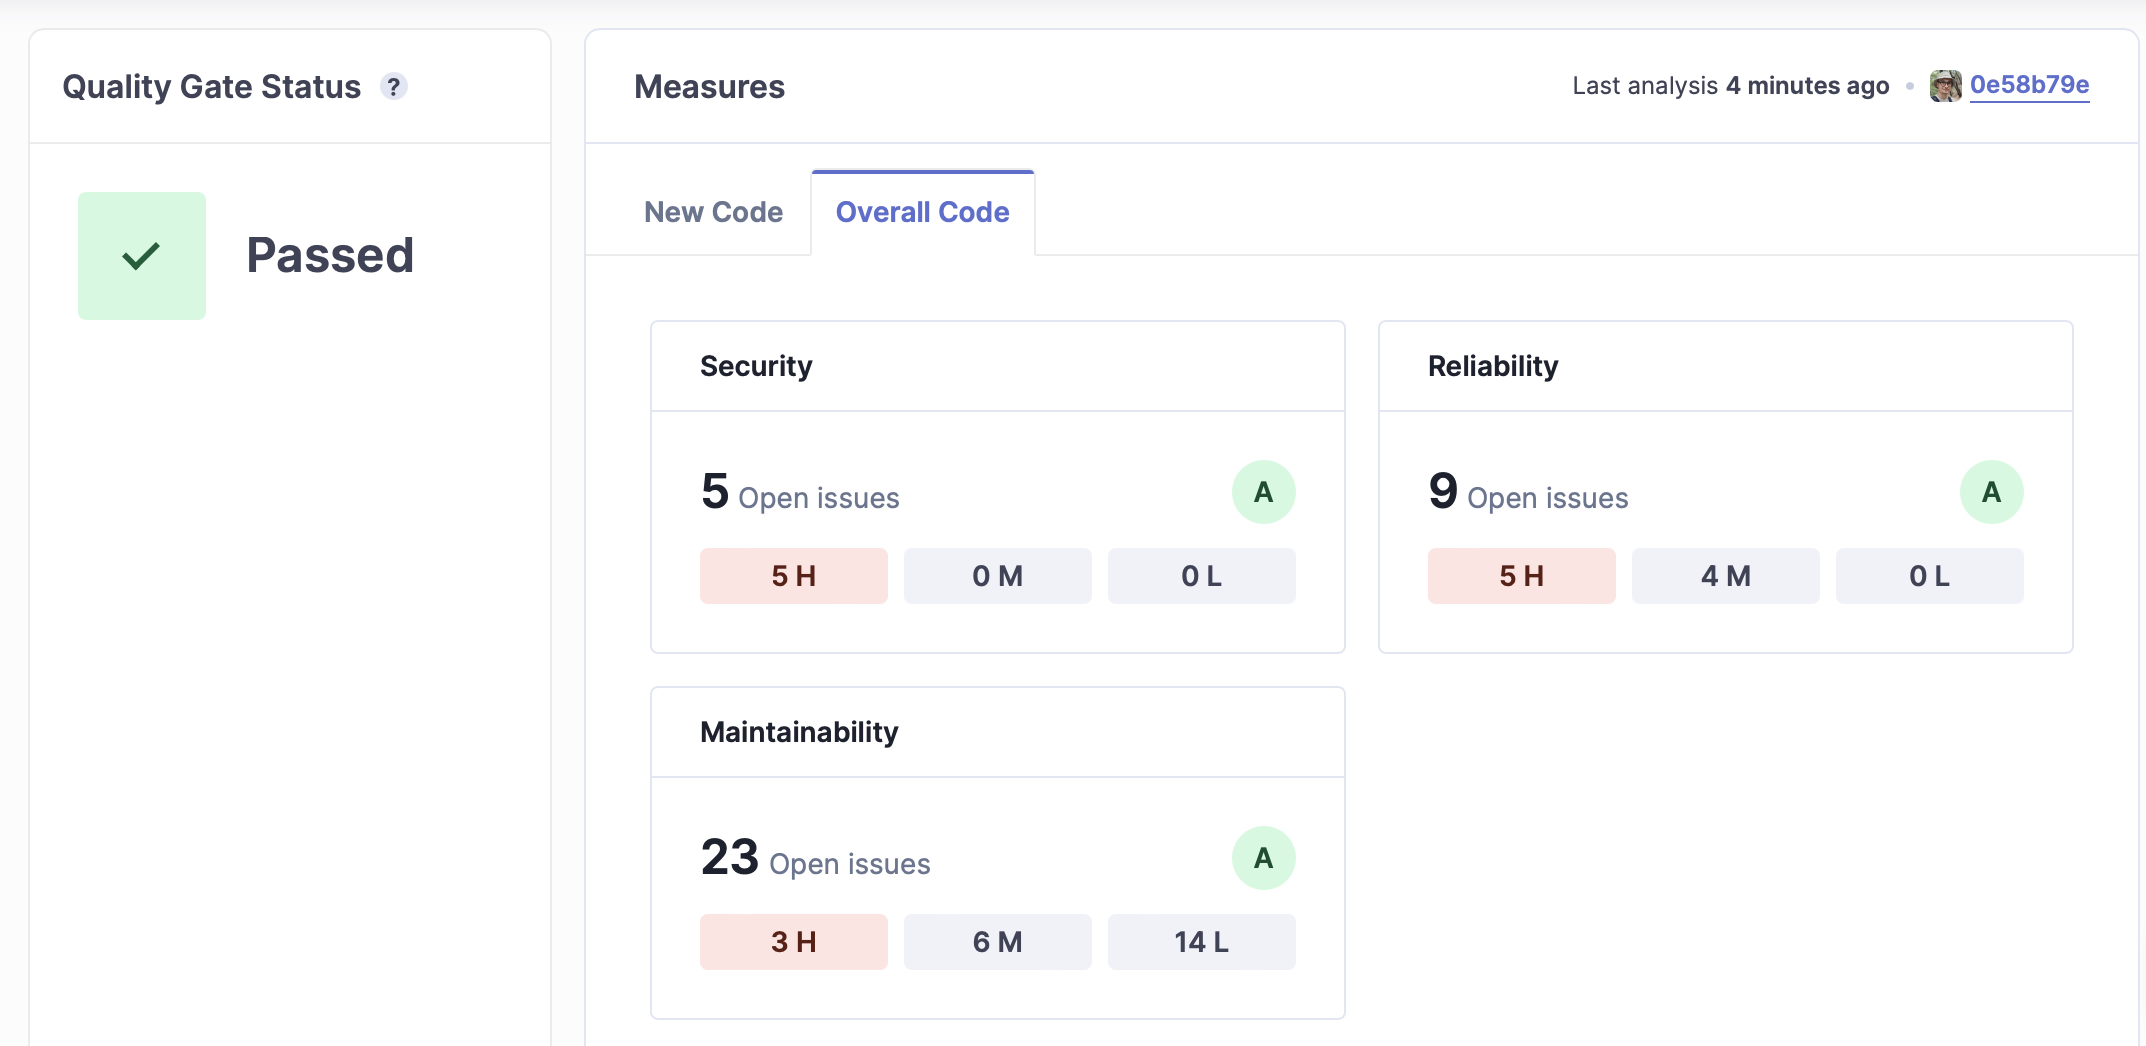
\includegraphics[width=\textwidth]{images/QualityGate.png}
    \caption{Screenshot of the latest SonarCloud Quality Gate}
    \label{img:qualitygate}
\end{figure}

\noindent Figure \ref{img:qualitygate} shows a screenshot of the latest quality gate state in SonarCloud. It displays, that there remains some open issues.  All of them have rating A, meaning that it has the lowest score when it comes to improving the software. \cite{codeclimate} When it comes to technical dept, we currently have 5\%, which improved after implementing the tools, as seen in Figure \ref{img:technical dept}. 

\begin{figure}[H]
    \centering
    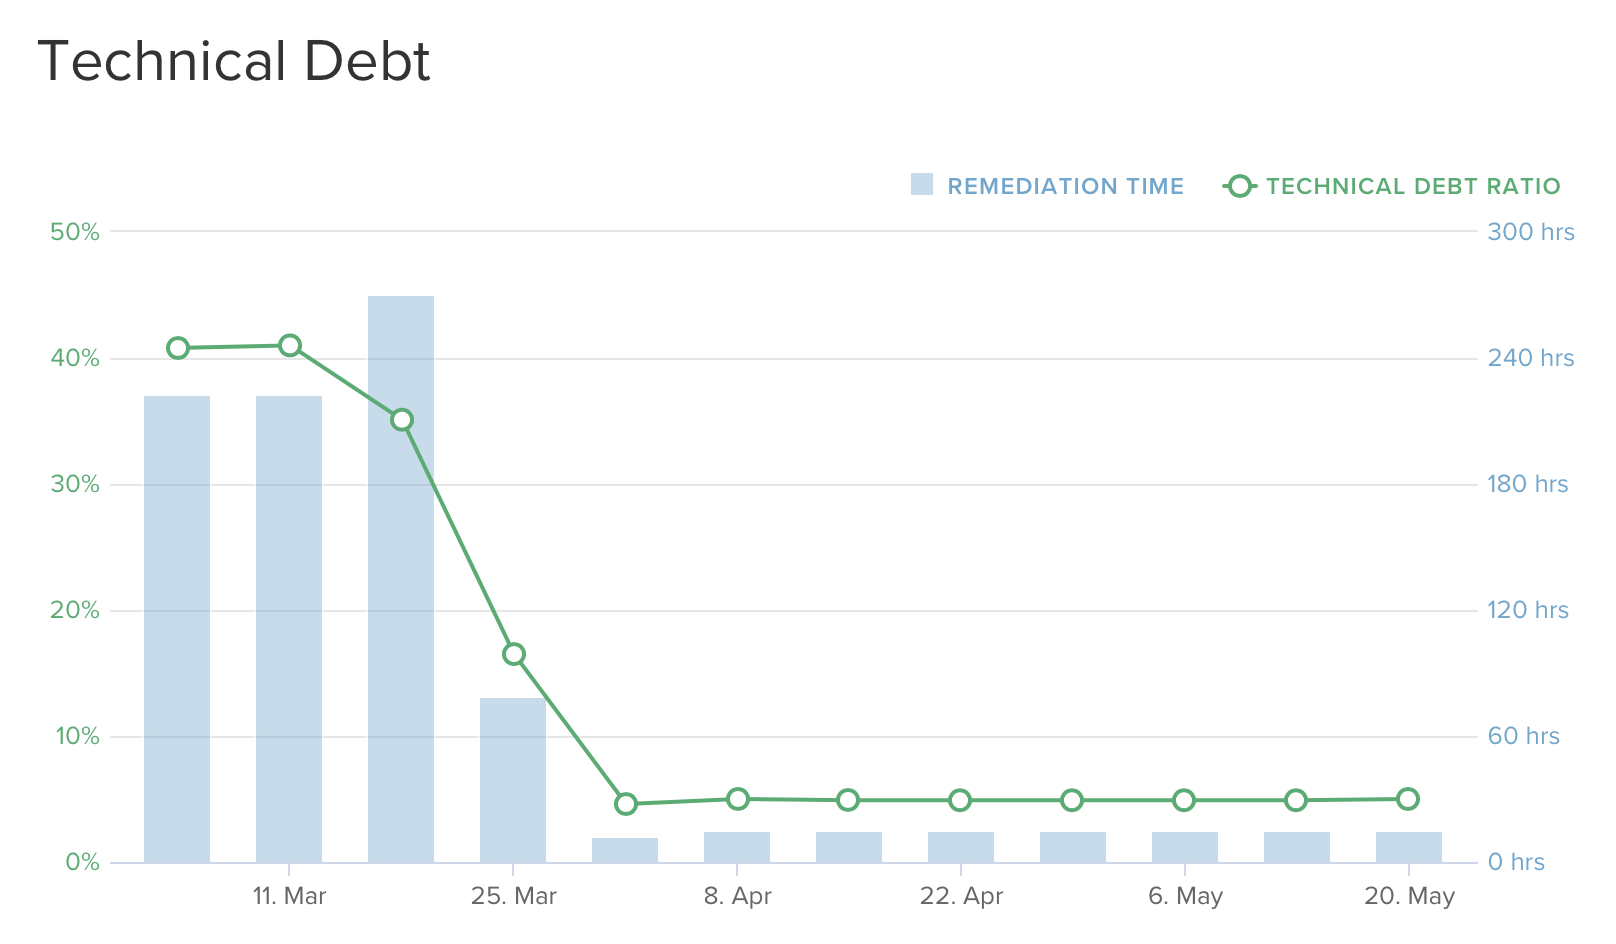
\includegraphics[width=\textwidth]{images/Technical Debt.png}
    \caption{Screenshot of the Technical Dept in our system, from CodeClimate}
    \label{img:technical dept}
\end{figure}


